\documentclass[10pt]{article}

\def\Type{LessonCaelan}
\def\TypeNum{Lesson 9}
\def\TypeTitle{Properties of Exponential \& Logarithmic Functions\\Notes To Instructors }
\def\Semester{Fall 2021} %Not Used 
\def\Course{MATH 1190 \& 1210}
\def\Targets{ {\bf \color{ProcessBlue}F2} }

\usepackage{preambleDJ}

\usepackage{ragged2e}

%%%%%%%%%%%% BEGIN DOCUMENT %%%%%%%%%%%%%%%
%%%%%%%%%%%% BEGIN DOCUMENT %%%%%%%%%%%%%%%
%%%%%%%%%%%% BEGIN DOCUMENT %%%%%%%%%%%%%%%
%%%%%%%%%%%% BEGIN DOCUMENT %%%%%%%%%%%%%%%
%%%%%%%%%%%% BEGIN DOCUMENT %%%%%%%%%%%%%%%

%%%%%%%%%%%% BEGIN DOCUMENT %%%%%%%%%%%%%%%
%%%%%%%%%%%% BEGIN DOCUMENT %%%%%%%%%%%%%%%
%%%%%%%%%%%% BEGIN DOCUMENT %%%%%%%%%%%%%%%
%%%%%%%%%%%% BEGIN DOCUMENT %%%%%%%%%%%%%%%
%%%%%%%%%%%% BEGIN DOCUMENT %%%%%%%%%%%%%%%

\begin{document}

\pagestyle{otherpages}
\thispagestyle{firstpage}
\vs{.6}

\paragraph*{Lesson Goals} related to target {\bf\color{ProcessBlue} F2: Exponential \& Logarithmic Functions}
\begin{itemize}
    \item Apply the properties of exponents and logarithms to simplify an expression. 
    \item Find the values of logarithmic expressions.
    \item Know properties of exponential and logarithmic function to find their domain, range, and common limits.
    \item solve equations involving exponential and logarithmic functions.
\end{itemize}


{\it Specific feedback from Pre-Class:}
\begin{itemize}
\item ``I found it interesting that logs, which seem very difficult and abstract, are actually just exponents."
\item ``The beginning made a lot of sense since I learned this before, however, it got a little confusing pretty fast once we had to actually quickly calculate the logs/ln."
    \begin{itemize}
    \item DJ's note: some students may never have interacted with logarithms without a calculator before. So, these students may not really know how logarithms relate to exponents.
    \end{itemize}
\item ``Could you go over this problem in class from the last video? $\ln(e-1) + \ln(e^2+e) - \ln(e^4-e^2)$. I was confused on how to simplify it completely."
    \begin{itemize}
    \item DJ's note: this is the last task in the pre-class lesson, and exactly Example 3 in the in-class lesson.
    \end{itemize}
\end{itemize}

{\it Handout structure:}
\begin{itemize}
\item {\bf\color{blue}Example 1} is an extension of the first video of the pre-class assignment, in which students see each of the properties of exponents used separately, but not altogether. The purpose of this example is:
    \begin{itemize}
    \item to show students what each of the rules look like in use; and
    \item to give students a quick example of how they might organize their work.
    \end{itemize}
You might physically point to the rules as you use them in your solution. This should take no more than a couple of minutes. 
\item {\bf\color{blue}Exercise A} is an immediate application of the rules you demonstrated in {\bf\color{blue} Example 1}.
    \begin{itemize}
    \item In part (a), they should know how the square root operation can be represented as an exponent from several prior lessons, but they may not know when to use this alternate representation.
    \item In part (b), students frequently want to move $2x$ down to the denominator as if the exponent $-4$ on the $x$ applied to both terms in some way.
    \item In part (c), watch out for the {\color{blue}\href{https://en.wikipedia.org/wiki/Freshman%27s_dream}{freshman's dream}}. This part was put here to remind students that a whole-number exponent indicates how many copies of something you're multiplying together.
    \end{itemize} 
\item {\bf\color{blue} Example 2} / {\bf\color{blue} Exercise B} corresponds directly to skills in the second video of the pre-class assignment. Use these tasks to help build the connection between logarithms and exponents - and to discourage students' tendencies to think of these objects as sets of completely unrelated tricks and algorithms.
    \begin{itemize}
    \item It's not uncommon for students to report having absolutely no exposure to logarithms, or to having last seen logarithms several years ago (and not understanding them then).
    \item That said, feel free to convert this entirely to an exercise if you feel your students don't need to see another model of how to approach this problem. Just make a copy of the lesson code, and delete the example command on that line, as well as the ``({\bf\color{blue} Example})" text.
    \end{itemize}
\item {\bf\color{blue} Example 3} / {\bf\color{blue} Exercise C} correspond directly to skills in the fourth video of the pre-class assignment relating to condensing logarithmic expressions.
    \begin{itemize}
    \item Students tend to struggle with these kinds of problems, particularly with how to interact productively with log properties at the top of the page.
    \item Try to physically point to the rule you're using as you use it in Example 3 so they'll think to look atop the page when solving Exercise C.
    \end{itemize}
\item {\bf\color{blue} Exercise D and E} Help students get familiarized with the shapes, domain and range of exponential and logarithmic functions. Note the derivative part will be taught in next Lesson. For now, encourage students make conjectures about the derivatives as much as they are able to. Try to hint them toward finding derivative functions that capture properties of the original function.
\item {\bf\color{blue} Exercise F} is an important exercise in helping students connect exponents and logarithms via the inverse function property. Students are presented with erroneous work done while solving an exponential or logarithmic equation, and then asked to identify \& correct mistakes.
    \begin{itemize}
    \item In part (a), different logarithms are erroneously applied to each side of the equation $2^{3-2/x}=10^x$ to simplify.
    \item In part (b), the exponential function of base 3 is ``distributed" across the addition on the left-hand side, rather than log properties being used first to combine before exponentiating.
    \end{itemize}
\item {\bf\color{blue} Exam Practice 1} reviews Exercises B, C, \& D. With practice, students tend to pick up how to do part (c), which pertains to the specific algorithm used to solve Exercise D, part (b). However, students struggle with parts (a) and (b), which pertain to simplification, as these parts are not viewed as a repeatable algorithm to many students.
%\item {\bf\color{blue} Extra Practice 1} is an extension of Exercise C, part (b). Students will need to use logarithm properties and factor strategically to complete the task.
\item {\bf\color{blue} Extra Practice 2} is a challenging extension of Exercise D in which students can (hopefully) more readily see the parallels in how one solves exponential \& logarithmic equations. 
    \begin{itemize}
    \item Parts (a) and (b) should be simpler applications of Exercise D. 
    \item However, parts (c) and (d) are particularly challenging, as part (c) uses the difference rule for logarithms - rather than the sum rule as in Exercise D part (a) - and as part (d) expects students to write $5^{x+2}-5^x$ as $5^{x}\cdot5^2 - 5^x$ and then factor to obtain $5^x\cdot(25-1)=24\cdot5^x$ before solving.
    \end{itemize}
\end{itemize}
\newpage

\textbf{Intended Learning Outcomes}
After this lesson, you will be able to 

\begin{itemize}
    \item Apply the properties of exponents and logarithms to simplify an expression. (\target{F2})
    \item Find the values of logarithmic expressions. (\target{F2})
    \item Know properties of exponential and logarithmic function to find their domain, range, and common limits. (\target{F2})
    \item solve equations involving exponential and logarithmic functions. (\target{F2})
\end{itemize}

\vspace{-0.5cm}

\hrulefill


{\bf Properties of Exponents}



\,\hfill
\fbox{$a^x=\underbrace{a\cdot a\cdot a\cdots a}_{x\text{ copies}}$}
\hfill
\fbox{$a^x a^y = a^{x+y}$}
\hfill
\fbox{$(a^x)^y = a^{xy}$}
\hfill
\fbox{$a^{x/y}=\sqrt[y]{a^x}$}
\hfill
\,\\

\,\hfill\hfill
\fbox{$a^{-x} = \dfrac{1}{a^x}$}
\hfill
\fbox{$\dfrac{a^x}{a^y}=a^{x-y}\text{ or }\dfrac{1}{a^{y-x}}$}
\hfill
\fbox{$\left( \dfrac{a}{b} \right)^z = \dfrac{a^{z}}{b^{z}}$}
\hfill\hfill\,


% when whole numbers, exponents indicate the number of copies of the base being multiplied together -> properties of exponents

\example{\color{ProcessBlue}F2} Simplify the expression below by rewriting exponential expression to contain only positive exponents, expanding exponential expressions (when possible), and using properties of multiplication and division.\\

$\left( \dfrac{ 2^{-3}e^4 }{ 2e^3 } \right)^2$

\important{Solution to {\bf\color{blue}Example 1}}
{
\blue{\[\left( \dfrac{ 2^{-3}e^4 }{ 2e^3 } \right)^2 = \left( \dfrac{ e^{4-3} }{ 2\cdot2^{3} } \right)^2 = \left( \dfrac{ e }{ 2^{1+3} } \right)^2 = \left( \dfrac{ e }{ 2^4 } \right)\cdot\left( \dfrac{ e }{ 2^4 } \right) = \dfrac{ e^{1+1} }{ 2^{4+4} } = \fbox{$\dfrac{e^2}{2^8}$}\]
}}

\exercise{\color{ProcessBlue}F2} Simplify each expression below by rewriting exponential expression to contain only positive exponents, expanding exponential expressions, and using properties of multiplication and division.

\begin{enumerate}
\item[(a)] $\sqrt{\dfrac{ e^{7} }{ e^{11} }}$
\end{enumerate}

\important{Solution to {\bf\color{blue}Exercise 2} (a)}
{
\blue{\[\sqrt{\dfrac{ e^{7} }{ e^{11} }} = \left(e^{7-11}\right)^{1/2} = \left(e^{-4}\right)^{1/2} = e^{-4\cdot\frac12} = e^{-2} = \fbox{$\dfrac1{e^2}$}\]
}}

\begin{enumerate}
\item[(b)] $\dfrac{ 2x^{-4}\sqrt{x^{3}} }{ 2^{-5}x^{1/2} }$
\end{enumerate}

\important{Solution to {\bf\color{blue}Exercise 2} (b)}
{
\blue{\[
\dfrac{ 2x^{-4}\sqrt{x^{3}} }{ 2^{-5}x^{1/2} } 
= 
\dfrac{2^{1-(-5)}\cdot x^{3/2}}{x^4x^{1/2}} 
= 
\dfrac{2^6}{x^{4+\frac12}x^{-3/2}}
=
\fbox{$\dfrac{64}{x^3}$}
\]
}}

\begin{enumerate}
\item[(c)] $(a+b)^2$
\end{enumerate}

\important{Solution to {\bf\color{blue}Exercise 2} (c)}
{
\blue{\[
(a+b)^2 = \underbrace{(a+b)\cdot(a+b)}_{2\text{ copies}} = \underset{F}{a^2}+\underset{O}{ab}+\underset{I}{ba}+\underset{L}{b^2} = \fbox{$a^2+2ab+b^2$}
\]
}}

%%%%%%%%%
%\newpage%
%%%%%%%%%

\begin{center}
({\it Properties of Logarithms})
\end{center}

\,\hfill 
\fbox{$\log_a(x)=b$ means $a^b = x$}
\hfill
\fbox{\begin{minipage}{0.11\textwidth}\begin{center}$\log_a(a^x)=x$\\[0.05in] $a^{\log_a(x)}=x$\end{center}\end{minipage}}
\hfill\,\\

\,\hfill
\fbox{$\log_a(x)+\log_a(y)=\log_a(xy)$}
\hfill
\fbox{$\log_a(x)-\log_a(y)=\log_a\left(\dfrac{x}{y}\right)$}
\hfill
\fbox{$p\log_a(x)=\log_a(x^p)$}
\hfill\,

% logarithms indicate the power to which the base must be raised in order to obtain the input -> properties of logarithms

\example{\color{ProcessBlue}F2} / \exercise{\color{ProcessBlue}F2} Evaluate the following:\\

\begin{minipage}[t][4in]{0.45\textwidth}
\begin{enumerate}
\item[(a)] ({\bf\color{blue}Example}) $\log_2\left( 8\right)$
    \important{Solution to {\bf\color{blue}Example 2} part (a)}
    {
    \blue{$\log_2(8)$ is the power to which we must raise $2$ in order to get $8$. $8=2^3$, so $\log_2(8)=\fbox{$3$}$.
    }}

\item[(b)] ({\bf\color{blue}Example}) $\ln\left( \dfrac{1}{\sqrt{e}} \right)$
    \important{Solution to {\bf\color{blue}Example 2} part (b)}
    {
    \blue{$\ln\left(\dfrac{1}{\sqrt{e}}\right)$ is the power to which we must raise $e$ in order to get $\dfrac{1}{\sqrt{e}}$. $\dfrac{1}{\sqrt{e}}=\dfrac{1}{e^{1/2}}=e^{-1/2}$, so $\ln\left(\dfrac{1}{\sqrt{e}}\right)=\fbox{$-\dfrac12$}$.
    }}

\end{enumerate}
\end{minipage}
%
\hfill
%
\begin{minipage}[t][4in]{0.45\textwidth}
\begin{enumerate}
\item[(c)] ({\bf\color{blue}Exercise}) $\log_5\left(\sqrt[3]{25}\right)$
    \important{Solution to {\bf\color{blue}Exercise B} part (c)}
    {
    \blue{$\log_5(\sqrt[3]{25})$ is the power to which we must raise $5$ in order to get $\sqrt[3]{25}$. $\sqrt[3]{25}=25^{1/3}=(5^2)^{1/3}=5^{2/3}$, so $\log_5(\sqrt[3]{25})=\fbox{$\dfrac23$}$.
    }}

\item[(d)] ({\bf\color{blue}Exercise}) $\ln\left( \dfrac{e^5}{e^7}\right)$
    \important{Solution to {\bf\color{blue}Exercise B} part (d)}
    {
    \blue{$\ln\left( \dfrac{e^5}{e^7}\right)$ is the power to which we must raise $e$ in order to get $\dfrac{e^5}{e^7}$. $\dfrac{e^5}{e^7}=e^{5-7}=e^{-2}$, so $\ln\left( \dfrac{e^5}{e^7}\right)=\fbox{$-2$}$.
    }}

\end{enumerate}
\end{minipage}

\example{\color{ProcessBlue}F2} Condense \& simplify the following logarithmic expression completely:\\ 

$\ln(e-1) + \ln(e^2+e) - \ln(e^4-e^2)$

    \important{Solution to {\bf\color{blue}Example 3}}
    {
    \blue{\begin{align*}
    \ln(e-1) + \ln(e^2+e) - \ln(e^4-e^2) &= \ln((e-1)(e^2+e)) - \ln(e^4-e^2) &\text{add first 2 logs as a product}\\
    &= \ln\left( \dfrac{(e-1)(e^2+e)}{(e^4-e^2)} \right) &\text{subtract the last log as a quotient}\\
    &= \ln\left( \dfrac{(e-1)\cdot e(e+1)}{e^2(e^2-1)}\right) &\text{extract common factors to simplify}\\
    &= \ln\left( \dfrac{e^1(e-1)(e+1)}{e^2(e-1)(e+1)}\right) &\text{factor }e^2-1\text{ as }(e-1)(e+1)\\
    &= \ln( e^{1-2} ) = \fbox{$-1$} &\text{divide away common factors \& solve}
    \end{align*}
    }}

%%%%%%%%%
%\newpage%
%%%%%%%%%
    
\exercise{\color{ProcessBlue}F2} Condense \& simplify the following logarithmic expressions completely:
\begin{enumerate}
\item[(a)] $\log_5 50+\log_5 7-\log_5 14$
\end{enumerate}
    \important{Solution to {\bf\color{blue}Exercise C} part (a)}
    {
    \blue{\begin{align*}
    \log_5 50+\log_5 7-\log_5 14 &= \log_5(50\cdot7)-\log_5(14) &\text{add first 2 logs as a product}\\
    &=\log_5\left( \dfrac{50\cdot7}{14}\right) &\text{subtract the last log as a quotient}\\
    &=\log_5\left( \dfrac{50}{2} \right) &\text{divide 14 by 7 to leave 2}\\
    &=\log_5(25) = \fbox{$2$} &\text{cancel common factors and solve}
    \end{align*}
    }}
\begin{enumerate}
\item[(b)] $\ln(e^2+e)-\ln(e^2-1)+\ln(e^2-e)$\\[0.3in]
\end{enumerate}
    \important{Solution to {\bf\color{blue}Exercise C} part (b)}
    {
    \blue{\begin{align*}
    \ln(e^2+e)-\ln(e^2-1)+\ln(e^2-e) &= \ln\left(\dfrac{e^2+e}{e^2-1}\right) + \ln(e^2-e) &\text{subtract first 2 logs as a quotient}\\
    &=\ln\left(\frac{(e^2+e)(e^2-e)}{e^2-1}\right) &\text{add the last log as a product}\\
    &=\ln\left(\frac{e(e+1)\cdot e(e-1)}{(e+1)(e-1)}\right) &\text{factor out common factors, }e^2-1\text{ as }(e+1)(e-1)\\
    &=\ln(e^2) = \fbox{$2$} &\text{cancel common factors and solve}
    \end{align*}
    }}

%%%%%%%%%
\newpage%
%%%%%%%%%

{\bf Exponential Functions}

%\setlength{\baselineskip}{18pt}
The behavior of an exponential function $a^x$ depends upon  the base $a$. Let's experiment and see if we can make a conjecture, i.e. an educated guess, about how the base impacts the graph of an exponential function. Let's start by sketching the graphs of $f(x)=2^x$ and $\ds g(x)=\left(\frac12\right)^x$.

%\setlength{\baselineskip}{12pt}

\exercise{\color{ProcessBlue}F2} Fill in the tables of values below, then sketch the graphs of $f(x)=2^x$ and $\ds g(x)=\left(\frac12\right)^x$. Answer the prompts that follow.\\
\def\sz{0.15in}
\mpageTth{.33}{.33}{.33}{
    \begin{center}
        \begin{tabular}{ c | c }
        $x$ & $f(x)=2^x$\\[0.05in]
        \hline
            & \\[-0.1in]
        $3$ & \blue{$8$} \\[\sz]
        $2$ & \blue{$4$}\\[\sz]
        $1$ & \blue{$2$}\\[\sz]
        $0$ & \blue{$1$}\\[\sz]
        $-1$ & \blue{$\dfrac{1}{2}$}\\[\sz]
        $-2$ & \blue{$\dfrac{1}{4}$}\\[\sz]
        $-3$ & \blue{$\dfrac{1}{8}$}\\[\sz]
        \end{tabular}
    \end{center}
}{
    \begin{center}
        \begin{tikzpicture}
        \begin{axis}[
        xlabel={$x$},
        xlabel style={anchor=west},
        xtick       = {-3,-2,-1,1,2,3},
        xticklabels = {$-3$,$-2$,$-1$,$1$,$2$,$3$},
        ytick       = {-3,-2,-1,1,2,3,4,5,6,7,8,9,10},
        yticklabels = { ,$-2$, , ,$2$, ,$4$, ,$6$, ,$8$, ,$10$},
        samples     = 320,
        domain      = -3.5:3.5,
        %restrict y to domain=-2.5:4.5,
        xmin = -3.5, xmax = 3.5,
        ymin = -0.5, ymax = 10.5,
        width = 2.1in, height = 3in,
        grid=both, grid style=dashed
        ]
        \filldraw[blue] (3,8) circle (2.5pt);
        \filldraw[blue] (2,4) circle (2.5pt);
        \filldraw[blue] (1,2) circle (2.5pt);
        \filldraw[blue] (0,1) circle (2.5pt);
        \filldraw[blue] (-1,.5) circle (2.5pt);
        \filldraw[blue] (-2,.25) circle (2.5pt);
        \filldraw[blue] (-3,.125) circle (2.5pt);
        \draw[domain=-3.4:3.35, color=blue, ultra thick, <->]   plot (\x,{2^(\x)})    node[right] {$f(x) = 2^x$};
          \filldraw[red] (-3,8) circle (2.5pt);        
        \filldraw[red] (-2,4) circle (2.5pt);
        \filldraw[red] (-1,2) circle (2.5pt);
        \filldraw[red] (0,1) circle (2.5pt);
        \filldraw[red] (1,.5) circle (2.5pt);
        \filldraw[red] (2,.25) circle (2.5pt);
        \filldraw[red] (3,.125) circle (2.5pt);
        \draw[domain=-3.35:3.4, color=red, ultra thick, <->]   plot (\x,{(1/2)^(\x)})    node[right] {$g(x) = \left(\dfrac{1}{2}\right)^x$};
        \node at (-1.5,8.75) {\footnotesize \red{$\ds y=\left(\frac{1}{2}\right)^x$}};
                \node at (2,8.75) {\footnotesize \blue{$\ds y=2^x$}};
        \end{axis}
        \end{tikzpicture}
    \end{center}
}{
    \begin{center}
        \begin{tabular}{ c | c }
        $x$ & $g(x)=\left(\frac12\right)^x$\\[0.05in]
        \hline
            & \\[-0.1in]
        $3$ & \red{$\dfrac{1}{8}$}\\[\sz]
        $2$ & \red{$\dfrac{1}{4}$}\\[\sz]
        $1$ & \red{$\dfrac{1}{2}$}\\[\sz]
        $0$ & \red{$1$}\\[\sz]
        $-1$ & \red{$2$}\\[\sz]
        $-2$ & \red{$4$}\\[\sz]
        $-3$ & \red{$8$} \\[\sz]
        \end{tabular}
    \end{center}
}
\vs{.1}~\\
{\bf  \blue{Conjecture/ Educated Guessing }} Consider our sketching exercise and make an educated guess about the behavior of $f(x)=a^x$. \\
\vs{-.3}
\mpageT{.45}{.45}[\hs{.35}]{
\enumA{
\item When $f(x)=a^x$ and  base $\mathbf{a>1}$, does the graph appear to increase to infinity or decrease to $0$ as $x$ gets larger? \label{eqn1}\\
\blue{Increase to infinity.}
\item When $f(x)=a^x$ and  base $\mathbf{0<a<1}$, does the graph appear to increase to infinity or decrease to $0$ as $x$ gets larger?\label{eqn2}
}
\blue{Decrease to $0$.}
}{
 {\em Conjecture} Based on your response in \ref{eqn1} and \ref{eqn2} what are some reasonable things you might say about each of the following symbols? Consider how the words above might translate to mathematical statements.\\\\
   \renewcommand{\arraystretch}{2.5} 
 \begin{tabularx}{1.3\textwidth}{| L{.3} L{.25} | L{.3} L{.25} |}     \hline
%\multicolumn{1}{c}{$a>1$} & \multicolumn{1}{x}{$0<a<1$}\\
\multicolumn{2}{ |C{.5} | }{$\mathbf{a>1}$ }&  \multicolumn{2}{ C{.5} | }{ $\mathbf{0<a<1}$} \\ \hline
$\bullet$   $f^{\prime}(x)$  & \unline{.5}{\blue{$>0$}}{.25} & $\bullet$   $f^{\prime}(x)$ & \unline{.5}{\blue{$<0$}}{.25} \\
$\bullet$   $\ds \lim_{x\to \infty}a^x=$  & \unline{.5}{\blue{$\infty$}}{.25}  & $\bullet$ $\ds \lim_{x\to \infty}a^x=$  & \unline{.5}{\blue{$0$}}{.25}\\
$\bullet$   $\ds \lim_{x\to -\infty}a^x=$ &  \unline{.5}{\blue{$0$}}{.25}  & $\bullet$ $\ds \lim_{x\to -\infty}a^x=$  & \unline{.5}{\blue{$\infty$}}{.25} \vs{.2}\\  \hline
%& &&\\ \hline
\end{tabularx}
  \renewcommand{\arraystretch}{1} 
}
\mpageT{.5}{.5}{
{\bf \blue{Exponential Functions}} 
\itemI{
\item $y=f(x)=a^x$\\
\blue{We assume $a>0$.\\ For example $3^x$, $e^x$, $\left(\dfrac{1}{4}\right)^x$, etc.}
\\
\item Domain (i.e. inputs): \blue{ $(-\infty, \infty)$}\\\\
\item Range (i.e. outputs): \blue{ $(0, \infty)$}\\
}
}{
{\bf \blue{Power Functions}}
\itemI{
\item $y=f(x)=x^a$\\
\blue{For example $x^2$, $x^5$, $\sqrt{x}=x^{1/2}$, etc.}
\\
\item Domain (i.e. inputs): \\
 \blue{ if $a$ is a non-negative integer, $(-\infty, \infty)$}
 \\
\item Range (i.e. outputs):\\
 \blue{ if $a$ is a negative {\em odd} integer, $(-\infty, \infty)$.   }\\
  \blue{ if $a$ is a negative {\em even} integer,  $[0, \infty)$. }\\
}
}
\newpage
%\item {\em Conjecture} Based on your response in \ref{eqn1} and \ref{eqn2} what are some reasonable things you might say about each of the following symbols? Consider how the words above might translate to mathematical statements.
{\bf Logarithmic Functions}

The behavior of a logarithmic function $\ds \log_a(x)$  depends upon  the base $a$. Let's experiment and see if we can make a conjecture, i.e. an educated guess, about how the base impacts the graph of an exponential function. Let's start by sketching the graph of $f(x)=\log_2(x)$.

\exercise{\bf\color{ProcessBlue}F2} Fill in the table of values below, then sketch the graph of $f(x)=\log_2(x)$. Answer the prompts that follow.

\mpageT{.33}{.67}{
    \begin{center}
        \begin{tabular}{ c | c }
        $x$ & $f(x)=\log_2(x)$\\[0.05in]
        \hline
            & \\[-0.1in]
        $1/8$ & \blue{$-3$} \\[\sz]
        $1/4$ & \blue{$-2$} \\[\sz]
        $1/2$ & \blue{$-1$} \\[\sz]
        $1$ &  \blue{$0$}\\[\sz]
        $2$ & \blue{$1$} \\[\sz]
        $4$ & \blue{$2$} \\[\sz]
        $8$ &\blue{$3$} \\[\sz]
        \end{tabular}
    \end{center}
}{
    \begin{center}
        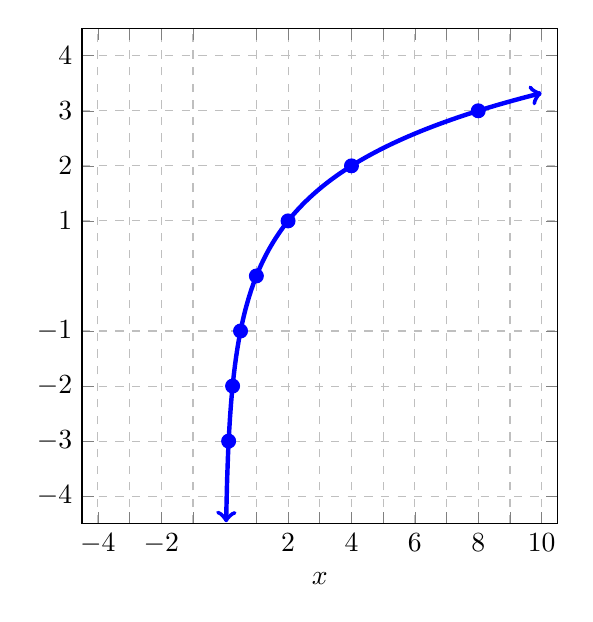
\begin{tikzpicture}
        \begin{axis}[
        xlabel={$x$},
        ytick       = {-4,-3,-2,-1,1,2,3,4},
        yticklabels = {$-4$,$-3$,$-2$,$-1$,$1$,$2$,$3$,$4$},
        xtick       = {-4,-3,-2,-1,1,2,3,4,5,6,7,8,9,10},
        xticklabels = { $-4$,,$-2$, , ,$2$, ,$4$, ,$6$, ,$8$, ,$10$},
        samples     = 320,
        domain      = -4.5:4.5,
        %restrict y to domain=-2.5:4.5,
        xmin = -4.5, xmax = 10.5,
        ymin = -4.5, ymax = 4.5,
        width = 3in, height = 3.1in,
        grid=both, grid style=dashed
        ]
        \filldraw[blue] (1/8,-3) circle (2.5pt);
        \filldraw[blue] (1/4,-2) circle (2.5pt);
        \filldraw[blue] (1/2,-1) circle (2.5pt);
        \filldraw[blue] (1,0) circle (2.5pt);
        \filldraw[blue] (2, 1) circle (2.5pt);
        \filldraw[blue] (4,2) circle (2.5pt);
        \filldraw[blue] (8,3) circle (2.5pt);
           \addplot[domain=0.045:10, blue, ultra thick, <->] {ln(x)/ln(2)};
        %\draw[color=blue, ultra thick]   plot ( \x,{ln(\x) } )  ;
        \node at (-1.5,8.75) {\footnotesize \red{$\ds y=\left(\frac{1}{2}\right)^x$}};
        \end{axis}
        \end{tikzpicture}
    \end{center}
}
\vs{.2}~\\
{\bf  \blue{Conjecture/ Educated Guessing }} Consider our sketching exercise and make an educated guess about the behavior of $f(x)=\log_a (x)$. \\
\vs{-.3}
\mpageT{.45}{.45}[\hs{.35}]{
\enumA{
\item When $f(x)=\log_a^x$ and  base $\mathbf{a>1}$, does the graph appear to increase to infinity, increase to negative infinity or decrease to $0$ as $x$ gets larger? \label{eqn3}\\
\blue{increases to $\infty$}
\vs{.5}
\item As $x$ gets closer to $0$, does the graph appear to increase to infinity, increase to negative infinity or decrease to $0$?\label{eqn4}\\
\blue{decreases to $-\infty$}
}
}{
 {\em Conjecture} Based on your response in \ref{eqn3} and \ref{eqn4} what are some reasonable things you might say about each of the following symbols? Consider how the words above might translate to mathematical statements.\\\\
  \renewcommand{\arraystretch}{2.5} 
 \begin{tabularx}{1.2\textwidth}{| L{.4} L{.25} | L{.25} L{.2} |}     \hline
\multicolumn{4}{ |C{1} | }{$\qquad \qquad \mathbf{f(x)=\log_a(x),\qquad a>1}$}  \\ \hline
$\bullet$   $f^{\prime}(x)$  &\unline{.5}{\blue{$>0$}}{.25} & $\bullet$   $\log_a(0)$ & \unline{.5}{\blue{$DNE$}}{.25} \\
$\bullet$   $\ds \lim_{x\to \infty} \log_a(x)=$  & \unline{.5}{\blue{$\infty$}}{.25}  & $\bullet$ $\ds \log_a(-3)$  & \unline{.5}{\blue{$DNE$}}{.25}\\
$\bullet$   $\ds \lim_{x\to 0^+} \log_a(x)=$ &  \unline{.5}{\blue{$\infty$}}{.25}   &    & \vs{.2}\\ \hline
%%& &&\\ \hline
\end{tabularx}
  \renewcommand{\arraystretch}{1} 
}
\vs{.25}\\
{\bf \blue{Logarithmic functions}}
\tasksI{3}{
\task $y=f(x)=\log_a(x)$\\
\blue{For example,\\ $\log_2(x)$, $\ln(x)=\log_e(x)$, $\log_{10}(x)$, etc.}
\\
\task Domain (i.e. inputs):\\
\blue{$(0,\infty)$}\\
\task Range (i.e. outputs):\\
\blue{$(-\infty,\infty)$}
}
{\em Key Idea: Inverse} 
\\
\blue{$a^x$ and $\log_a(x)$ are inverse functions. This means they ``reverse" the action of the other. Mathematically, this means $$a^{\log_a(x)}=x \text{ and }\log_a(a^x)=x$$}
%%%%%%%%%
\newpage%
%%%%%%%%%

\example{\color{ProcessBlue}F2} Solve the following equations for $x$.
%
\begin{enumerate}
\item[(a)] $2^{3-2x} = 10^x$

% {\color{red}
% \begin{align*}
% 2^{3-2x} &= 10^x\\
% \log_2\left(2^{3-2x}\right) &= \log_{10}(10^x) &\text{applied a log to both sides}\\
% 3-2x &= x &\text{used log properties to simplify}\\
% 3 &= 3x &\text{added }2x\text{ to both sides}\\
% x &= 1 &\text{divided both sides by 3}
% \end{align*}
% }
\end{enumerate}

\important{Solution to {\bf\color{blue}Exercise D} part (a)}
    {
    %The mistake lies in the second line when logarithms were applied to both sides of the equation. To maintain equality, we must do the {\it same} thing to both sides, so we cannot apply different logarithms to both sides of the equation. Instead, just pick a single logarithm to apply to both sides, and then solve.

    \blue{\begin{align*}
    2^{3-2x} = 10^x &\implies \log_2(2^{3-2x}) = \log_2(10^x) &\text{applied }\log_2\text{ to both sides}\\
    &\implies 3-2x = x\log_2(10) &\text{used log properties to simplify}\\
    &\implies 3=x\log_2(10)+2x &\text{added }2x\text{ to both sides}\\
    &\implies 3=x(\log_2(10)+2) &\text{factored common factor of }x\text{ on right side}\\
    &\implies x=\fbox{$\dfrac{3}{\log_2(10)+2}$}&\text{divided both sides by }\log_2(10)+2
    \end{align*}
    }}

%%%%%%%%%
%\newpage%
%%%%%%%%%

\begin{enumerate}
\item[(b)] $\log_3(x+4)+\log_3(x-2)=3$

% {\color{red}
% \begin{align*}
% \log_3(x+4)+\log_3(x-2) &= 3\\
% 3^{\log_3(x+4)+\log_3(x-2)} & = 3^3 &\text{exponentiated both sides, using base of }3\\
% (x+4) + (x-2) &= 27 &\text{used log properties to simplify}\\
% 2x+2 &= 27 &\text{combined like terms}\\
% 2x &= 25 &\text{subtracted }2\text{ from both sides}\\
% x &= \frac{25}2 &\text{divided both sides by }2
% \end{align*}
% }
\end{enumerate}

\important{Solution to {\bf\color{blue}Exercise D} part (b)}
    {
    %The mistake lies in the third line, where a log property was used incorrectly to simplify. The property being invoked is $a^{\log_a(x)}=x$. To apply this property, we would need to resolve the addition of logarithms in some way, either by using logarithm or exponential properties.

    \blue{\begin{align*}
    \log_3(x+4)+\log_3(x-2)=3 &\implies \log_3\left((x+4)(x-2)\right) = 3\\
    &\implies 3^{\log_3((x+4)(x-2))} = 3^3\\
    &\implies (x+4)(x-2) = 27\\
    &\implies x^2-2x+4x-8 = 27\\
    &\implies x^2+2x-35 = 0\\
    &\implies (x+7)(x-5) = 0\\
    &\implies x=-7,\,5
    \end{align*}

    The original equation involved logarithms, which are undefined when their inputs are not positive. So, we need to check whether these values make the inputs of the logarithms negative or zero.\\

    {\bf Case:} $x=-7$

    \[\log_3(-7+4)+\log_3(-7-2)=3 \quad \implies \quad \log_3(-3) + \log_3(-9) = 3 \quad\implies\quad \text{undefined!} \]

    So, $x=-7$ can't be a solution as it causes the original equation to be undefined.\\

    {\bf Case:} $x=5$

    \[\log_3(5+4)+\log_3(5-2)=3 \quad\implies\quad \log_3(9)+\log_3(3)=3 \quad\implies\quad \log_3(27)=3\]

    \fbox{$x=5$} is the solution, as it satisfies the original equation.
    }}
%%%%%%%%%
\newpage%
%%%%%%%%%

The following problem appeared on an assessment during the Fall 2023 semester.\\

{\bf\color{blue}Exam Practice 1.} \reversemarginpar \marginnote{\fbox{\bf\color{ProcessBlue}F2}}
%
Respond to the following prompts.
\begin{enumerate}
    
        \item[(a)] Evaluate: \quad $\displaystyle \log_{2} \left( \frac{1}{32} \right)=$\unline{1}{\blue{$-5$}}
        \sol{
        \al{
        \log_{2} \left( \frac{1}{32} \right)&=\log_{2} \left( \frac{1}{2^5} \right)\\
        &=\log_2(2^{-5})\\
        &=-5 \qquad \text{ (since $\log_2(x)$ and $2^x$ are inverse functions of each other).}
        }
        }
        
        \item[(b)] Simplify the expression completely: \quad $\displaystyle e^{3 \ln( 5)} - \ln( e ) + \frac{\ln( e^3)}{\ln( e^5)} - \ln( e^3 e^5) $
        \sol{
        Note:
        \itemI{
        \item $\ds e^{3 \ln( 5)}=e^{\ln(5^3)}=5^3=125$
        \item $\ds \ln(e)=\ln(e^1)=1$
        \item $\ds  \frac{\ln( e^3)}{\ln( e^5)}= \frac{3\ln( e)}{5\ln( e)}=\frac{3}{5}$
        \item $\ds  \ln( e^3 e^5)=\ln(e^3)+\ln(e^5)=3+5=8$
        }
        We put all this together and 
        \al{
        e^{3 \ln( 5)} - \ln( e ) + \frac{\ln( e^3)}{\ln( e^5)} - \ln( e^3 e^5) &=125-1+\frac{3}{5}-8\\
        &=116\frac{3}{5}
        }
        }
        
 
    
        \item[(c)] Solve the following equation for $x$: \quad $\displaystyle \log_2(x - 3) + \log_2(x + 1) = 5$
\sol{
\al{
\log_2(x - 3) + \log_2(x + 1) &= 5\\
\log_2 \left((x-3)(x+1)\right)&=5 \\
2^{\log_2 \left((x-3)(x+1)\right)}&=2^5\\
(x-3)(x+1)&=32\\
x^2-2x-3&=32
x^2-2x-35&=0\\
(x-7)(x+5)&=0\\
}
Thus $x=7$ or $x=-5$.  Notice that
\itemI{
\item  $x=7$ {\em is} in the domain since $\log_2(7 - 3)=\log_2(4)=\log_2(2^2)=2$ is defined and  $\log_2(7 + 1)=\log_2(8)=\log_2(2^3)=3$ is also defined.
\item $x=-5$ {\em is not} in the domain since $\log_2(x - 3)=\log_2(-5-3)=\log_2(-8)$ is not defined.
}
Thus $x=7$ is the only solution.
} 

        \vfill
       
    \end{enumerate}

%{\bf\color{blue}Extra Practice 1.} \reversemarginpar \marginnote{\fbox{\bf\color{ProcessBlue}F2}} Condense and simplify the following logarithmic expression completely: \[2\log t+3\log (t+1)-\frac13\log(t^3+2t^2+t)\]

%\vfill
%\vfill

%%%%%%%%%
%\newpage%
%%%%%%%%%
{\bf\color{blue}Extra Practice 1.} \reversemarginpar \marginnote{\fbox{\bf\color{ProcessBlue}F2}}
%
Find all possible solutions to the following equations.
\begin{enumerate}
\item[(a)] $5^x-4=0$
    \sol{
    \al{
    5^x-4&=0\\
    5^x&=4\\
    \log_5(5^x)&=\log_5(4)\\
    x&=\log_5(4)\\
    x&\approx0.86
    }
    }
\item[(b)] $5^x+5=0$
\sol{
\al{
5^x+5&=0\\
5^x&=-5
}
But $5^x$ can never be negative and thus $5^x\neq-5$. This means there are not solutions.
}
\item[(c)] $5^{2x}+5^x-20=0$
  \sol{
  \al{
  5^{2x}+5^x-20&=0\\
  (5^x)^2+5^x-20&=0\\
  (5^x+5)(5^x-4)&=0
  }
  Thus either $5^x+5=0$ or $5^x-4=0$. We saw in (b) that $5^x+5=0$ has no solutions. \\
   We saw in part (a) that $5^x-4=0$ has solution $ x=\log_5(4)\approx0.86$.
  }
\item[(d)] $2e^{2x}-5e^x+2=0$
\sol{
\al{
2e^{2x}-5e^x+2&=0\\
2\left(e^{x}\right)^2-5e^x+2&=0\\
(2e^x-1)(e^x-2)&=0
}
Thus either $(2e^x-1)=0$ or $(e^x-2)=0$
\al{
2e^x-1&=0\\
2e^x=1\\
e^x&=\frac{1}{2}\\
\ln(e^x)&=\ln \left(\frac{1}{2}\right)\\
x&=\ln \left(\frac{1}{2}\right)\\
x&\approx-0.69
}
The other possibility is 
\al{
e^x-2&=0\\
e^x&=2\\
\ln(e^x)&=\ln(2)\\
x&=\ln(2)\\
x\approx 0.69
}
}
\end{enumerate}


\newpage
{\bf\color{blue}Extra Practice 2.} \reversemarginpar \marginnote{\fbox{\bf\color{ProcessBlue}F2}} 
%
Find all possible solutions to the following equations.
\begin{enumerate}
\item[(a)] $\log_5(x+2)-2=0$
\sol{
\al{
\log_5(x+2)-2&=0\\
\log_5(x+2)&=2\\
5^{\log_5(x+2)}&=5^2\\
x+2&=25\\
x&=23
}
$x=23$ {\em is} in the domain since $\log_5(x+2)=\log_5(23+2)$ is defined (i.e. no logarithm of $0$ or negative number) 
}

\item[(b)] $5^{x+2}-2=0$
 \sol{
 \al{
 5^{x+2}-2&=0\\
 5^{x+2}&=2\\
 \log_5(5^{x+2})&=\log_5(2)\\
 x+2&=\log_5(2)\\
 x&=\log_5(2)-2
 }
 }
\item[(c)] $\log_5(x+2)-2 = \log_5(x)$
\sol{
\al{
\log_5(x+2)-2 &= \log_5(x)\\
\log_5(x+2) - \log_5(x)&=2\\
\log_5\left(\frac{x+2}{x} \right)&=2\\
5^{\log_5\left(\frac{x+2}{x} \right)}&=5^2\\
\frac{x+2}{x}&=25\\
x+2=25x\\
2&=24x\\
\frac{2}{24}&=x\\
\frac{1}{12}&=x
}
}
\item[(d)] $5^{x+2}-2=5^{x}$
\sol{
\al{
5^{x+2}-2&=5^{x}\\
5^{x+2}-5^x&=2\\
5^x\cdot 5^2-5^x&=2\\
5^x\left(5^2-1\right)&=2\\
5^x&=\frac{1}{5^2-1}\\
5^x&=\frac{1}{24}\\
\log_5(5^x)&=\log_5\left(\frac{1}{24}\right)\\
x&=\log_5\left(\frac{1}{24}\right)\\
x&\approx -1.97
}
}
\end{enumerate}

\end{document}
